\subsection{La vision}

% ------------- %

\frame{
	\frametitle{Physiologie, neurobiologie et al.}

	Comment voyons nous ?
	
	\begin{itemize}[<+(1)->]
		\item L'oeil : une perception physiologique sans analyse.

		\item Le cerveau : analyse des données renvoyées par l'oeil.
	\end{itemize}
}


% ------------- %

\frame{
	\frametitle{Problèmes informatiques associés}
	
	Quatre problématiques.
	
	\begin{itemize}[<+(1)->]
		\item Représenter des images.

		\item Capter des images.

		\item Coder les images (à émettre ou captées).
		
		\item Analyser des images pour leur donner du sens.
	\end{itemize}
}


% ------------- %

\frame{
	\frametitle{Problématique 1 - Représenter des images}
	
	Nécessité de mieux connaître le fonctionnement de l'oeil.
	
	\pause
	
	\medskip
	
	Un fait important, les photorécepteurs : 
	les cônes et les bâtonnets.
	
	\begin{itemize}[<+(1)->]
		\item Les cônes pour la couleur - Intensité lumineuse correcte.
		
		\begin{itemize}[<+(1)->]
			\item Environ 7 millions principalement au centre de la rétine.
			
			\item Sensibles à trois type de couleurs : 
			
			      bleu (420 nm), vert (535 nm) et jaune-rouge (570 nm). 
		\end{itemize}

		\item Les bâtonnets - Faible intensité lumineuse.
		
		\begin{itemize}[<+(1)->]
			\item Environ 120 millions principalement en périphérie de la rétine.
			
			\item Incapables de différencier plusieurs teintes.
			
			\item Bien plus sensibles à la lumière que les cônes (vision nocturne).
		\end{itemize}
	\end{itemize}
}


% ------------- %

\frame{
	\frametitle{Problématique 1 - Représenter des images}
	
	Solution technique adoptée : 
	
	émission de lumières rouge, verte et bleue \og{}mélangées\fg{}.
	
	\pause

	\medskip
	
	De petits émetteurs pour chacune des trois couleurs.
	
	\begin{center}
		
\includegraphics[width=0.50\textwidth]{physiology/tv.jpg}
		
		{\scriptsize Photo en gros plan d'une télévision \\ \phantom{x}}
	\end{center}
}


% ------------- %

\frame{
	\frametitle{Problématique 1 - Représenter des images}
	
	\phantom{Solution technique adoptée : }
	
	\phantom{émission de lumières rouge, verte et bleue \og{}mélangées\fg{}}.

	\medskip
	
	\phantom{De petits émetteurs pour chacune des trois couleurs}.
	
	\begin{center}
		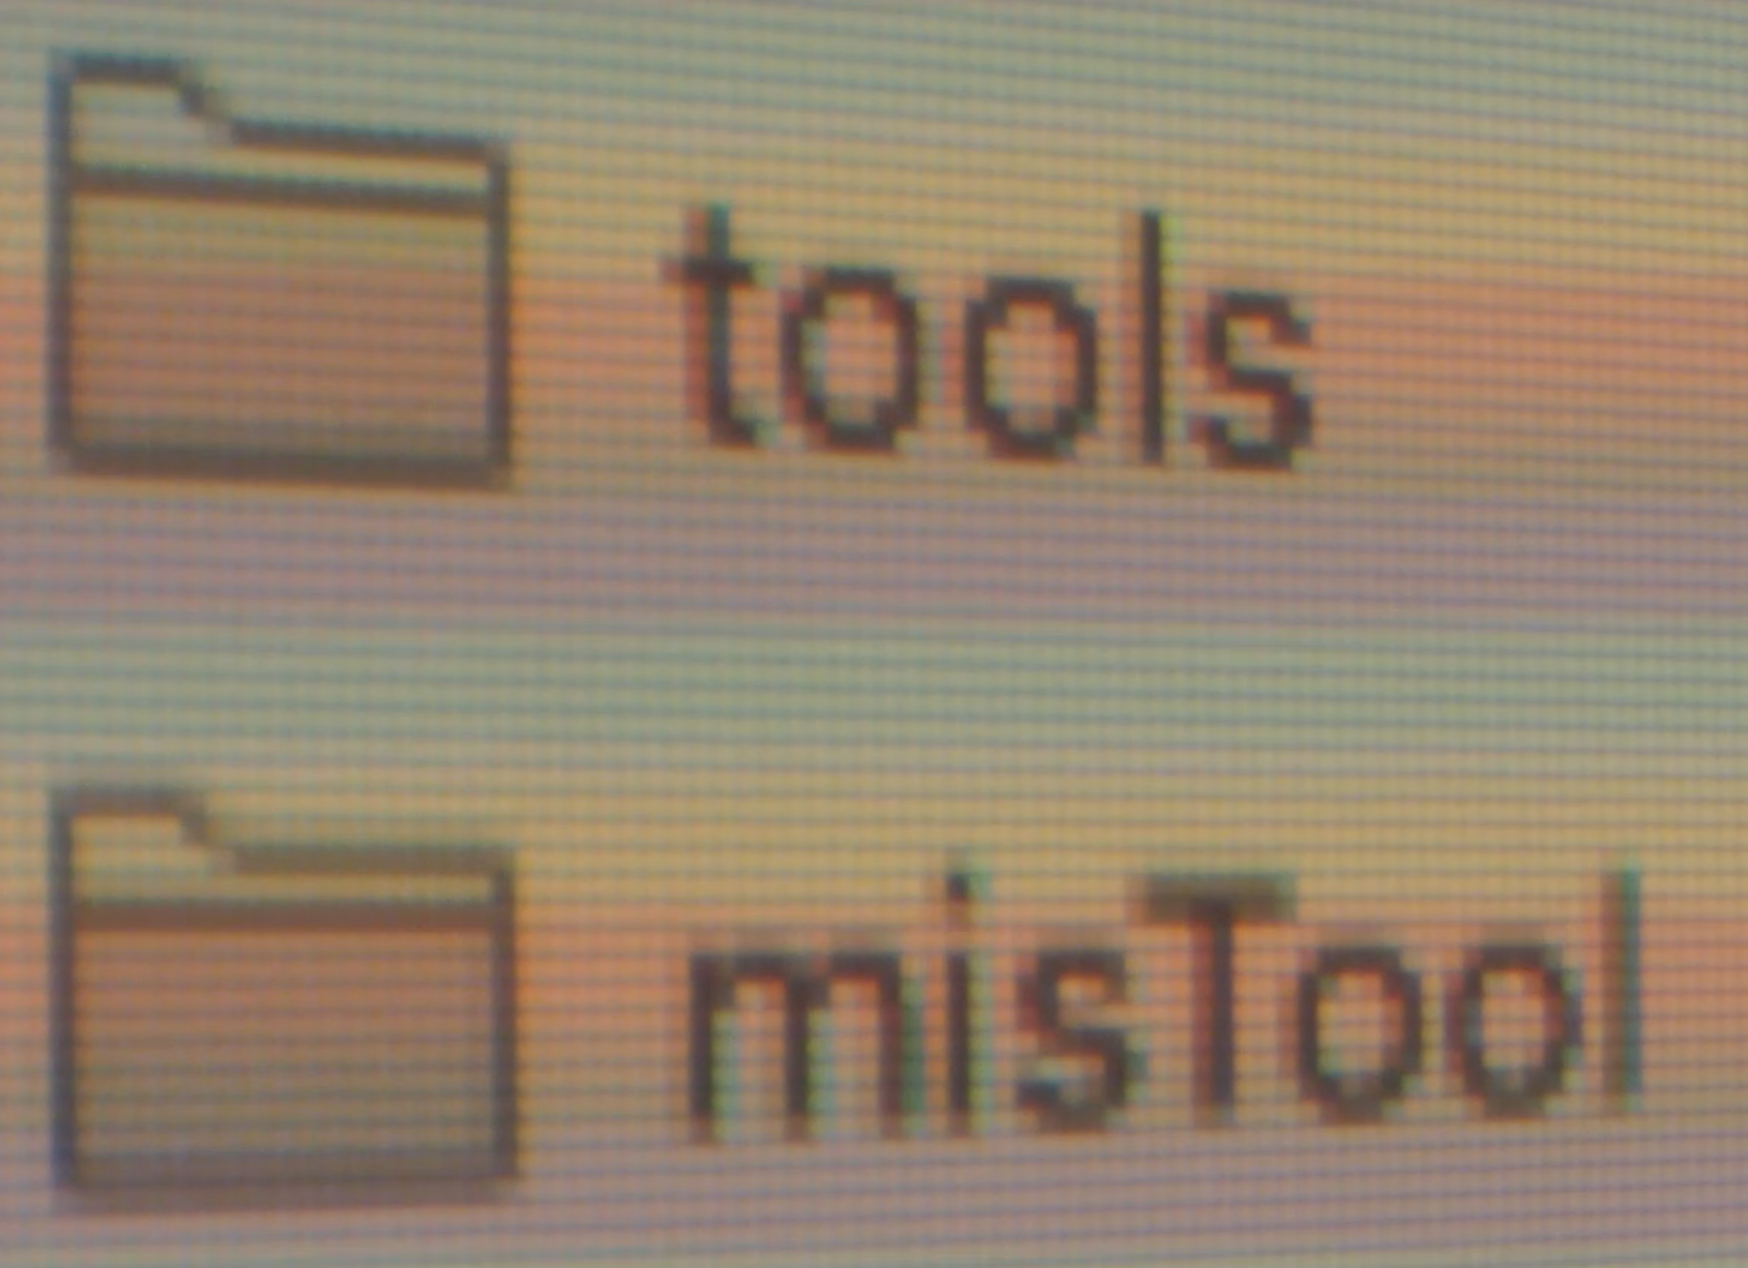
\includegraphics[width=0.50\textwidth]{physiology/videproj.png}
		
		{\scriptsize Image extraite d'une vidéo filmant le rendu d'un vidéo projecteur \\ (le fond était visuellement blanc)}
	\end{center}
}


% ------------- %

\frame{
	\frametitle{Problématique 2 - Capter des images}
	
	Principe \og{}inverse\fg{} de la représentation.
	
	\begin{itemize}[<+(1)->]
		\item Utilisation de petits capteurs spécialisés dans une couleur.
		
		\item Application des résultats de la physique quantique.
		
		\item Mesures électriques traduites en nombres.
	\end{itemize}
}


% ------------- %

\frame{
	\frametitle{Problématique 3 - Coder les images}
	
	\begin{itemize}[<+(1)->]
		\item Comment coder une image ?
		
		\item Quelles conventions utilisées ?
		
		\item Nécessité d'établir des standards.
	\end{itemize}
}


% ------------- %

\begin{frame}[fragile]
	\frametitle{Problématique 4 - Analyser des images}
	
	Problème difficile.
	\pause
	Pourquoi ?
	
	\pause
	
	\medskip 
	
	Imaginons que l'on code par $1$ le noir et $0$ le blanc.
	
	\pause
	
	\medskip 
	
	Seriez-vous me dire ce que représente l'image noir et blanc de dimension 13 \og{}cases\fg{} horizontalement sur 17 verticalement qui est codée ci-dessous ? 
	
	\begin{center}
		\scriptsize
		\begin{verbatim}
00000000000000000001000000000001110000000001010100000001000001000001
00000001000111000001110010111111101001001000100100100100010010010010
00100100100100010010010010001001001001000100100011000001100000111111
10000000000000000
		\end{verbatim}
	\end{center}
\end{frame}


% ------------- %

\begin{frame}[fragile]
	\frametitle{Problématique 4 - Analyser des images}
	
	Réorganisation des chiffres (respect des dimensions).
	
	\begin{center}
		\scriptsize
		\begin{verbatim}
0000000000000
0000001000000
0000011100000
0000101010000
0001000001000
0010000000100
0111000001110
0101111111010
0100100010010
0100100010010
0100100010010
0100100010010
0100100010010
0100100010010
0011000001100
0001111111000
0000000000000
		\end{verbatim}
	\end{center}
\end{frame}


% ------------- %

\frame{
	\frametitle{Problématique 4 - Analyser des images}
	
	Voici l'image (ajout du quadrillage pour les sceptiques).
	
	\begin{center}
		
\includegraphics[scale=0.15]{physiology/crayon.png}
	\end{center}
	
	On devine un crayon...	
	Pas si simple même en noir et blanc !
	
	\pause

	\medskip
	
	Imaginez les problématiques soulevées avec des images en couleur.
}


% ------------- %

\begin{frame}[fragile]
	\frametitle{Problématique 4 - Analyser des images}
	
	\textbf{Attention !} Codons par \verb+#+ le noir et par \verb+.+ le blanc.
	
	\medskip 
	
	On obtient visuellement un crayon.
	
	\begin{center}
		\scriptsize
		\begin{verbatim}
.............
......#......
.....###.....
....#.#.#....
...#.....#...
..#.......#..
.###.....###.
.#.#######.#.
.#..#...#..#.
.#..#...#..#.
.#..#...#..#.
.#..#...#..#.
.#..#...#..#.
.#..#...#..#.
..##.....##..
...#######...
.............
		\end{verbatim}
	\end{center}
\end{frame}


% ------------- %

\frame{
	\frametitle{Problématique 4 - Analyser des images}
	
	Ceci ne signifie pas que ce nouveau codage est meilleur.
	
	\medskip
	
	Pourquoi ?
	\pause
	Tout est dans le \og{}visuellement\fg{}. 
}


% ------------- %


\frame{
	\frametitle{Problématique 4 - Analyser des images}
	
	\begin{center}
		\framebox{\textbf{Ne pas oublier qu'un ordinateur est juste un calculateur !}}
	\end{center} 
}